\chapter{Objektorientierte Analyse}


\section{Lernziele}

\begin{itemize}
    \item für kleinere Projekte qualitätssichernde Maßnahmen planen und verfolgen können
    \item Tests planen und dokumentieren können
    \item gefundene Fehler geeignet verwalten können
\end{itemize}

\newpage


\section{Modelle in Analyse und Entwurf}

\subsection*{Analyse}

\vspace{2mm}
Die Analyse beschreibt fachliche Zusammenhänge, keine technischen.
\vspace{2mm}



Bereits in der ersten Phase der Softwareentwicklung gesammelte Anforderungen können nicht direkt umgesetzt werden, da sie meist viel zu ungenau sind.
Offene Punkte müßten durch einen dauernden Kontakt zu Endanwender und Kunde geklärt werden.\\
Außerdem zeigt sich, dass Anforderungen in sich widersprüchlich sein können, ohne, dass das auf den ersten Blick erkennbar ist.\\

\noindent
Eine Lösung wäre es, die Dokumente aus der Anforderungsphase sehr formal zu gestalten, wodurch die Dokumente aber sehr umfangreich und schwer verständlich werden.\\

\noindent
Stattdessen erstellt man in der \textbf{Analysephase} ein formales Modell sowohl des Problems \textit{in seinem Umfeld} als auch der Lösung.

\subsection*{Entwurf}
In der \textbf{Entwurfsphase} werden die \textbf{Architektur} der Anwendung bestimmt, unter Berücksichtung technischer Randbedingungen, die im Rahmen nicht-funktionaler Anforderungen in der Anforderungsphase gesammelt wurden und vom Kunden stammen (s. Abschnitt~\ref{subsec:technische-randbedingung}).\\
Die Architektur schließt u.a. ein:

\begin{itemize}
    \item Programmiersprache
    \item Frameworks
    \item Einsatz von Datenbanken
    \item \ldots
\end{itemize}

\noindent
Meist bleiben im Anschluss technische Fragen offen, die in der \textbf{Entwurfsphase} beantwortet werden.

\begin{itemize}
    \item Welche \textbf{Klassen} aus der \textbf{Analyse} können übernommen werden?
    \item Wie werden Klassen in einem relationalen Datenbank-Schema gespeichert?
    \item Welche Steuerungklassen müssen für die GUI implementiert werden?
\end{itemize}

\noindent
Das Erstellen eines Modells der geplanten Software bietet den Vorteil, das Entwurfs-Alternativen einfacher und schneller durchdacht werden können, und die Zusammenarbeit einfacher ist, wenn die Umsetzung genauer geplant wird (vgl. \cite[2]{Wed09b}).


\subsection*{Definition Modell}


\vspace{2mm}
\begin{tcolorbox}[title=Arbeitsdefinition ``Modell``]
    Ein \textbf{Modell} ist ein Produkt des \textbf{Modellierungsvorgangs}.\\

    \noindent
    Es beschriebt tatsächliche oder gedachte Gegenstände oder Konzepte und deren Beziehungen.\\

    \noindent
    Ein Modell erfasst diese Konzepte nicht vollständig, sondern \textbf{abstrakt}, also verkürzt und vereinfacht (vgl. \cite[2]{Wed09b}).
\end{tcolorbox}
\vspace{2mm}

\subsection*{Statische und dynamische Modelle}

\noindent
Modelle der Analyse und des Entwurfs bestehen aus miteinander verzahnten \textbf{statischen} und \textbf{dynamischen} Modellen:

\begin{itemize}
    \item \textbf{statische Modelle} beschreiben die Bausteine eines Systems und wie sie zusammengesetzt sind\footnote{vergleichbar mit technischen Zeichnungen}
    \item \textbf{dynamische Modelle} beschreiben die Zusammenarbeit der Bausteine, also deren verhalten und die Nachrichten, die Verhalten auslösen
\end{itemize}

\noindent
\textbf{Dynamische Modelle} sind \textit{notwendig}, da das Zusammenspiel der Modellelemente aus dem statischen Modell nicht immer eindeutig abgeleitet werden kann.\\

\noindent
Als Grundlage zur Modellierung wird meist der \textbf{objektorientierte} Ansatz gewählt\footnote{
    mit dem Vorteil, dass für die Modellierung dieselben Techniken gewählt werden wie bei der späteren Umsetzung
}.\\

\noindent
Hierfür wird i.d.R. \textbf{UML}\footnote{
s. UML Version 2.5.1: \url{https://www.omg.org/spec/UML/}, abgerufen 10.04.2024
} verwendet, damit die Beschreibung eindeutig für alle Benutzer ist.
\section{Klassen und Objekte}

\noindent
\textbf{Klassen} sind Abstraktionen von Objekten.\\

\noindent
\textbf{Objekte} besitzen Eigenschaften und Verhalten.\\

\noindent
In der \textbf{UML} werden Attribute und Verantwortlichkeiten oder Operationen in \textbf{Compartments} (dt. \textit{Abteilungen}) dargestellt.\\

\noindent
Einschränken des Typs können hinter dem Typ in geschweiften Klammern in der \textbf{Object Constraint Language}-Notation\footnote{
s. Version 2.4: \url{https://www.omg.org/spec/OCL}, abgerufen 11.04.2024
} (\textbf{OCL}) angegeben werden\footnote{
alternativ können Kommentare in entsprecheder UML-Notation angegeben werden.
}
Diese Angaben - oder als Kommentar in Textform angegeben - ersetzen im \textit{Klassendiagramm der Analyse} das \textbf{Datadictionary} (s. Abschnitt~\ref{sec:datadictionary-und-mengengerust}) (s. Abbildung~\ref{fig:moneyocl}).

\begin{figure}
    \centering
    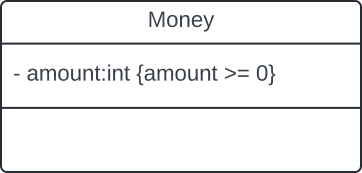
\includegraphics[scale=0.4]{part two/Objektorientierte Analyse/img/moneyocl}
    \caption{Die OCL-Notation in Verbindung mit einem UML-Klassendiagramm zur Spezifizierung des Wertebereichs des Attributes \textit{amount}. (Quelle: eigene)}
    \label{fig:moneyocl}
\end{figure}
\section{Beziehungen von Klassen}

Klassen können auf drei unterschiedliche Arten miteinander in Beziehung stehen:

\begin{itemize}
    \item \textbf{Abhängigkeit} \textit{Dependency}
    \item \textbf{Assoziation} \textit{Association}
    \item \textbf{Vererbung} \textit{Inheritance}
\end{itemize}

\noindent
Bei der Analyse müssen diese Arten von Beziehungen ermittelt werden, damit entsprechend modelliert werden kann.\\

\subsection*{Abhängigkeiten}
\textbf{Abhängikeiten} nutzten eine gestrichelte Linie.\\
Abhängigkeiten werden \textit{in der Analyse} i.d.R. selten modelliert.\\
Als Beispiel für eine Abhängigkeit sei eine \textit{Benutzt-Beziehungen} in Form eines \textit{formalen Parameter} gegeben: Der aktuelle Parameter überdauert den Aufruf einer Methode in einer Klasse, für die diese Abhängigkeit modelliert werden soll, nicht.\\
Gleicherweise kann auch eine \textit{lokale Variable} eines bestimmten Typs eine Abhängigkeit bedeuten.

\subsection*{Assoziation}
Unter einer \textbf{Assoziation} versteht man, dass ein Objekt ein anderes Objekt derselben oder anderen Klasse \textit{dauerhaft} kennt.\\
Assoziationen werden anhand einer durchgezogenen Linie dargestellt.\\
Wird in einem Objekt einer bestimmten Klasse in einem Attribute eine Referenz auf ein Objekt einer anderen oder derselben Klasse gespeichert, existiert eine Assoziation zwischen diesen beiden Klassen.

\subsection*{Vererbung}
Eine \textbf{Vererbung} bedeutet in Vererbungsrichtung eine \textbf{Spezialisierung}, entgegengesetzt eine \textbf{Generalisierung}\footnote{
bzw. \textit{Verallgemeinerung} im Skript (vgl.~\cite[7]{Wed09b}).
}.

\subsection*{Polymorphie}
Eine weitere Bedeutung der Vererbungsbeziehung, ist, dass eine Instanz einer Klasse genauso verwendet werden kann wie eine Instanz seiner übergeordneten Klasse. Allgemein faßt man dies unter \textbf{Polymorphie} zusammen.\\
Als Konsequenz folgt, dass immer dann, wenn ein bestimmter Typ gefordert wird, auch sein Untertyp erlaubt ist (vgl.~\cite[466]{Ull23}), was der Kern des \textit{Liskovschen Substitutionsprinzips}\footnote{
    ``Wikipedia - Liskov substitution principle``: \url{https://en.wikipedia.org/wiki/Liskov_substitution_principle}, abgerufen 11.04.2024
} ist\footnote{
    s.a. ``Wikipedia - Covariance and Contravariance``: \url{https://en.wikipedia.org/wiki/Covariance_and_contravariance_(computer_science)}, , abgerufen 11.04.2024
}.\\

\input{part two/Objektorientierte Analyse/domänenmodell}
\section{Modellierung der Dynamik}

\noindent
In der \textbf{statischen Modellierung} im Domänenmodell werden Klassen in ihrem \textit{Zusammenhang} modelliert.\\

\noindent
Das statische Modell gibt keine Informationen über den Zustand eines Objektes oder wie Botschaften untereinander ausgetauscht werden, und wie sich Objekte / Klassen daraufhin verhalten.\\

\noindent
Um darzustellen, wie sich Klassen oder Objekte verhalten, nutzt man das \textbf{dynamische Modell}.\\

\noindent
Hierzu werden in der \textbf{Analyse} Zustände und Zustandsübergänge eines Systems sowie Aktivitäten modelliert.\\
Grundlage sind Dokumente der Anforderungen, die \textbf{Verhalten} beschreiben, also\textbf{User Stories}, \textbf{Anwendungsfälle} und \textbf{Szenarien}.\\
Die dort beschriebenen Abläufe werden bei der dynamischen Modellierung konkretisiert und genauer definiert.

\subsection*{Zustände und Zustandsänderungen}
\textbf{Systeme} (\textit{Klassen}, \textit{Subsysteme}, \textit{Anwendungen}) können \textbf{Zustände} besitzen, die sich verändern können.\\

\noindent
Oft sind nur Übergänge zwischen bestimmten Zuständen möglich.\\

\noindent
Die grafische Darstellung dieses Verhaltens erreicht man über \textbf{UML-Zustandsdiagramme} (s. Abbildung~\ref{fig:statediagram}).

\begin{figure}
    \centering
    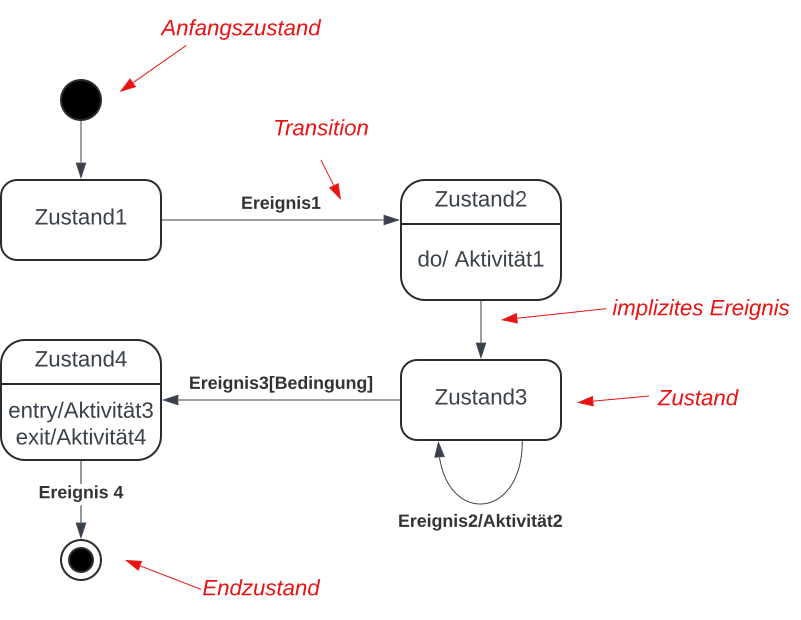
\includegraphics[scale=0.4]{part two/Objektorientierte Analyse/img/statediagram}
    \caption{In der Objektorientierung werden Zustandsautomaten mit Hilfe von Zustandsdiagrammen (\textit{statechart diagram}) dargestellt. Die in der Abbildung gezeigten /do/entry/exit-Aktivitäten werden innerhalb eines Zustands aufgerufen. Ein \textit{implizites Ereignis} (auch: \textit{Beendigungsereignis}) liegt vor, wenn die mit dem Vorgängerzustand verbundene Verarbeitung beendet ist, und eine \textit{Transition} in den Folgezustand führt. (Quelle: in Anlehnung an~\cite[90, Abb. 2.11-6]{Bal05})}
    \label{fig:statediagram}
\end{figure}

\subsection*{Aktivitätsdiagramme}
Bei Zustandsdiagrammen erschließt sich der Ablauf von Aktivitäten meist nur indirekt, da bspw. keine Auskunft über die beteiligten Akteure modelliert werden können.\\

\noindent
Aus diesem Grund verwendet man \textbf{UML-Aktivitätsdiagramm}, in denen Aktivitäten in ihrer möglichen Abfolge und ihrer Zuordnung zu Akteuren modelliert werden.\\

\noindent
Darüberhinaus kann mit Aktivitätsdiagrammen  auch der Fluss von Informationen un die Auswirkung auf Objekte dargestellt werden.\\

\vspace{2mm}
\begin{tcolorbox}
Aktivitätsdiagramme sind zur Modellierung von User Storys, Szenarien oder Anwendungsfällen geeignet.
\end{tcolorbox}
\vspace{2mm}
\section{Analysemuster}\label{sec:analysemuster}

\subsection*{Muster}
Im Software Engineering versteht man unter dem Begriff \textit{Muster} (\textit{Pattern}) \textbf{vorgefertigte Lösungsschablonen für verallgemeinerte Probleme}.\\

\noindent
Bei der Entwicklung tauchen häufig ähnliche Probleme auf, bei denen sich auch die Art der Lösung entsprechend ähnelt.\\

\noindent
Die Beschreibung der verallgemeinerten Probleme und Lösungen auf eine \textbf{formalisierte Weise} nennt man \textbf{Muster}.\\

\noindent
Muster müssen zur Anwendung auf ein konkretes Problem \textit{konkretisiert} werden.\\

\noindent
Im Bereich des Software Engineerings gibt es Muster für \textbf{Analyse}, \textbf{Architektur}, \textbf{Entwurf}.

\subsection*{Vorteile}

\begin{itemize}
    \item es stehen \textbf{bewährte Standardlösungen} zur Verfügung
    \item Verwendung bereits bewährter Lösungen ist oft \textbf{schneller und besser} als selbstentwickelte neue Lösungen
    \item Muster helfen bei der \textbf{Kommunikation}
\end{itemize}


\subsection*{Standardisierte Beschreibung}

\begin{itemize}
    \item Beschreibung des Problems in seinem Kontext
    \item Lösung
    \item Beispiele
    \item Gegebenenfalls Antimuster
\end{itemize}

\noindent
Eine Auswahl wichtigster Analysemuster in der o.a standardisierten Beschreibung findet sich in~\cite[22 ff.]{Wed09b} und wird im Folgenden verkürzt wiedergegeben.

\subsection{Exemplartyp (Abstraction - Occurence)}

\subsubsection*{Problem}
\begin{itemize}
    \item Objekte einer Klasse ähneln sich untereinander und tragen gemeinsamen, gleiche Informationen oder besitzen gleiches  Verhalten, unterscheiden sich aber wesentlich
    \item dieser Zusammenhang zwischen den Klassen soll zum Ausdruck gebracht werden
    \item es soll vermieden werden, dass mehrere Instanzen identische Daten mehrfach beinhalten
\end{itemize}

\subsubsection*{Lösung}
\begin{itemize}
    \item Gemeinsame Daten beinhalten Objekte der Klasse \code{Abstraction}
    \item individuelle Daten beinhalten Objekte der Klasse \code{Occurence}
\end{itemize}

\subsubsection*{Beispiel}
s. Abbildung~\ref{fig:abstractionoccurence}

\begin{figure}
    \centering
    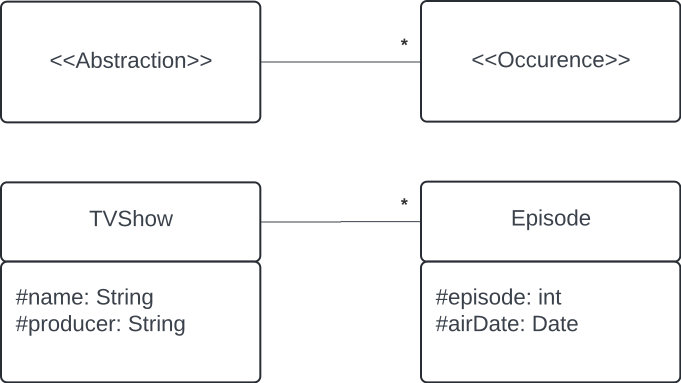
\includegraphics[scale=0.4]{part two/Objektorientierte Analyse/img/abstractionoccurence}
    \caption{Beispiel für das \textit{Abstraction-Occurence-Pattern}. (Quelle: eigene)}
    \label{fig:abstractionoccurence}
\end{figure}


\subsubsection*{Antipattern}
\begin{itemize}
    \item Alle Daten als Attribute einer Klasse modellieren (Zusammenhang von Klassen mit gleichen Daten wird nicht ausgedrückt)
    \item Vererbung (jedes Exemplar eine eigene Klasse)
\end{itemize}


\subsubsection*{Grenzen}
Kann nur sinnvoll eingesetzt werden, wenn die einzelnen Exemplare sinvoll unterschieden werden können, bspw. anhand einer \textbf{Identity}.



\subsection{Wechselnde Rollen (Player - Role)}

\subsubsection*{Problem}
\begin{itemize}
    \item ein Objekt kann in unterschiedlichen Kontexten verschiedene Verantwortlichkeiten und Beziehungen haben
    \item die Verantwortlichkeiten können sich ändern
\end{itemize}

\subsubsection*{Lösung}
\begin{itemize}
    \item Verantwortlichkeiten aus dem Objekt (\code{Player}) nehmen
    \item Verantwortlichkeiten in Objekte (\code{Role}) auslagern
    \item Konkrete Rollen erben von einer Rollensuperklasse
\end{itemize}

\subsubsection*{Beispiel}
s. Abbildung~\ref{fig:playerrole}

\begin{figure}
    \centering
    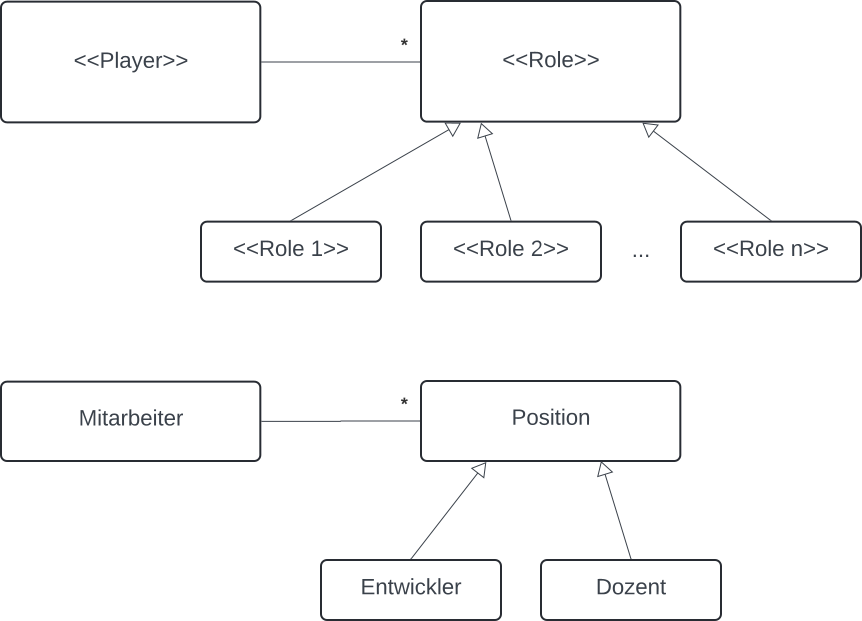
\includegraphics[scale=0.4]{part two/Objektorientierte Analyse/img/playerrole}
    \caption{Beispiel für das \textit{Player-Role-Pattern}. (Quelle: eigene)}
    \label{fig:playerrole}
\end{figure}


\subsubsection*{Antipattern}
\begin{itemize}
    \item Vererbung (eine Klasse identifiziert sich über den Typ der Rolle)
\end{itemize}


\subsection{Allgemeine Hierarchie (General Hierarchy, Kompositum)}

\subsubsection*{Problem}
\begin{itemize}
    \item Objekte können hierarchisch angeordnet sein
    \item Jedes Objekt kann maximal einem Objekt untergeordnet sein
    \item manche Objekte dieser Hierarchie können keine untergeordneten Objekte haben
\end{itemize}

\subsubsection*{Lösung}
\begin{itemize}
    \item Klassen werden von einer Superklasse \code{Node} abgeleitet
    \item Klassen, die andere Klassen referenzieren können, sog. \code{SuperiorNode}s, besitzen Referenzen auf \code{Node}s
    \item Klassen, die keine anderen Klassen referenzieren können, sind \code{NonSuperiorNodes}s
\end{itemize}

\subsubsection*{Beispiel}
s. Abbildung~\ref{fig:generalhierarchy}

\begin{figure}
    \centering
    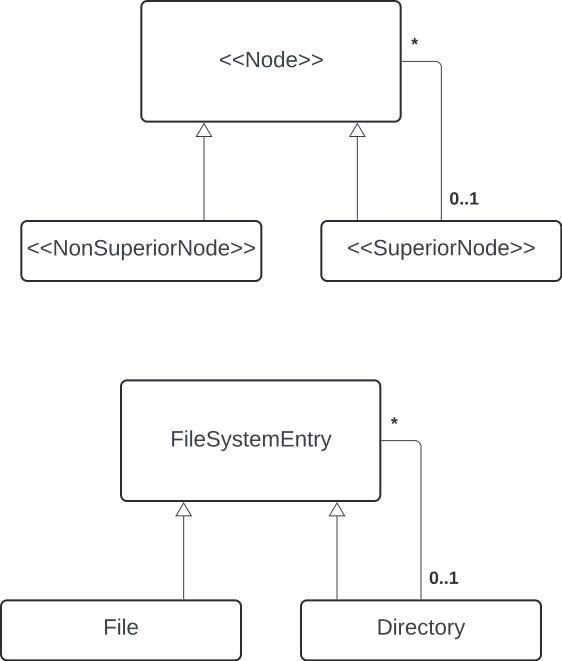
\includegraphics[scale=0.4]{part two/Objektorientierte Analyse/img/generalhierarchy}
    \caption{Beispiel für das \textit{General-Hierarchy-Pattern}. (Quelle: eigene)}
    \label{fig:generalhierarchy}
\end{figure}


\subsubsection*{Antipattern}
\begin{itemize}
    \item Vererbung: Die Vererbung beschreibt \textit{kann-verwendet-werden-als} oder auch \textit{ist-ein}, was bei einem Kompositum aber nicht immer zutrifft.
\end{itemize}


\begin{tcolorbox}
    \blockquote[{\cite[28, Hervorhebung eigene]{Wed09b}}]{
        Beim Muster \textit{Allgemeine Hierarchie} wird die Hierarchie von Objekten modelliert, nicht die Hierarchie von Klassen.
    }
\end{tcolorbox}



\newpage

